%\documentclass[10pt,notes]{beamer}       % print frame + notes
%\documentclass[10pt, notes=only]{beamer}   % only notes
\documentclass[11pt]{beamer}              % only frames

%%%%%% IF YOU WOULD LIKE TO CREATE LECTURE NOTES COMMENT OUT THE FOlLOWING TWO LINES
%\usepackage{pgfpages}
%\setbeameroption{show notes on second screen=bottom} % Both

\usepackage{graphicx}
\DeclareGraphicsExtensions{.pdf,.png,.jpg}
\usepackage{color}
\usetheme{winslab}
\usepackage[utf8]{inputenc}
\usepackage[english]{babel}
\usepackage{amsmath}
\usepackage{amsfonts}
\usepackage{amssymb}




\usepackage{algorithm2e,algorithmicx,algpseudocode}
\algnewcommand\Input{\item[\textbf{Input:}]}%
\algnewcommand\Output{\item[\textbf{Output:}]}%
\newcommand\tab[1][1cm]{\hspace*{#1}}

\algnewcommand{\Implement}[2]{\item[\textbf{Implements:}] #1 \textbf{Instance}: #2}%
\algnewcommand{\Use}[2]{\item[\textbf{Uses:}] #1 \textbf{Instance}: #2}%
\algnewcommand{\Trigger}[1]{\Statex{\textbf{Trigger:} (#1)}}%
\algnewcommand{\Events}[1]{\item[\textbf{Events:}] #1}%
\algnewcommand{\Need}[1]{\item[\textbf{Needs:}] #1}%
\algnewcommand{\Event}[2]{\Statex \item[\textbf{On#1:}](#2) \textbf{do}}%
\algnewcommand{\Trig}[3]{\State \textbf{Trigger}  #1.#2 (#3) }%
\def\true{\textbf{T}}
\def\false{\textbf{F}}


\author[Yağızcan Pançak]{Yağızcan Pançak\\\href{mailto:yagizcan.pancak@metu.edu.tr}{yagizcan.pancak@metu.edu.tr}}
%\author[J.\,Doe \& J.\,Doe]
%{%
%  \texorpdfstring{
%    \begin{columns}%[onlytextwidth]
%      \column{.45\linewidth}
%      \centering
%      John Doe\\
%      \href{mailto:john@example.com}{john@example.com}
%      \column{.45\linewidth}
%      \centering
%      Jane Doe\\
%      \href{mailto:jane.doe@example.com}{jane.doe@example.com}
%    \end{columns}
%  }
%  {John Doe \& Jane Doe}
%}

\title[Commit Protocols]{Commit Protocols}
\subtitle[SubTitle]{Two-Phase (2PC) and Three-Phase (3PC) Commit Protocols}
%\date{} 

\begin{document}

\begin{frame}[plain]
\titlepage
\note{In this talk, I will present .... Please answer the following questions:
\begin{enumerate}
\item Why are you giving presentation?
\item What is your desired outcome?
\item What does the audience already know  about your topic?
\item What are their interests?
\item What are key points?
\end{enumerate}
}
\end{frame}

\begin{frame}[label=toc]
    \frametitle{Outline of the Presentation}
    \tableofcontents[subsubsectionstyle=hide]
\note{ The possible outline of a talk can be as follows.
\begin{enumerate}
\item Outline 
\item Problem and background
\item Design and methods
\item Major findings
\item Conclusion and recommendations 
\end{enumerate} Please select meaningful section headings that represent the content rather than generic terms such as ``the problem''. Employ top-down structure: from general to more specific.
}
\end{frame}
%
%\part{This the First Part of the Presentation}
%\begin{frame}
%        \partpage
%\end{frame}
%
\section{Fault Tolerance in Distributed Systems}
%\begin{frame}
%        \sectionpage
%\end{frame}

\begin{frame}{Distributed Commit Problem}
\framesubtitle{The distributed commit problem refers to ensuring that all nodes in a distributed system either commit or abort a transaction together, preventing inconsistencies in data across the system.}
\begin{block}{One-Phase Commit Protocol} 
Distributed commit is often established by a coordinator. In a simple
scheme, this coordinator tells all other processes that are also involved, called
participants, whether to (locally) perform the operation in question. This
scheme is referred to as a \textbf{one-phase commit protocol}. The drawback is that if one of the participants cannot actually perform the operation,
there is no way to tell the coordinator.
\end{block}
\note{}
\end{frame}

\section{The Contribution: Two-Phase Commit Protocol (2PC)}
\begin{frame}
\frametitle{Two-Phase Commit Protocol (2PC)}
\framesubtitle{}
The Two-Phase Commit Protocol (2PC) ensures atomicity in distributed transactions efficiently. 

\begin{figure}
    \centering
    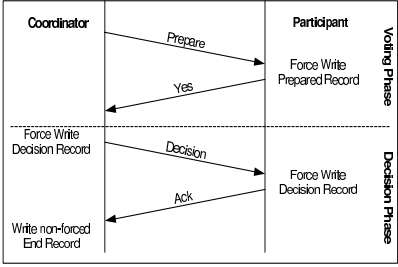
\includegraphics[scale=0.3]{figures/2PC.png}
    \caption{Two-Phase Commit Protocol (2PC)}
    \label{fig:2pc}
\end{figure}
\begin{itemize}
\item Offers a systematic approach for achieving atomicity.
\item Coordinates between a coordinator and participants.
\item Coordinator sends "prepare" message, participants respond.
\item Coordinator makes decision, sends "commit" or "abort".
\item Guarantees atomicity, minimizes inconsistencies.
\end{itemize}

\end{frame}

\section{The Contribution: Three-Phase Commit Protocol (3PC)}
\begin{frame}
\frametitle{Three-Phase Commit Protocol (3PC)}
\framesubtitle{}
The Three-Phase Commit Protocol (3PC) enhances distributed transaction atomicity with an additional phase for improved fault tolerance.

\begin{figure}
    \centering
    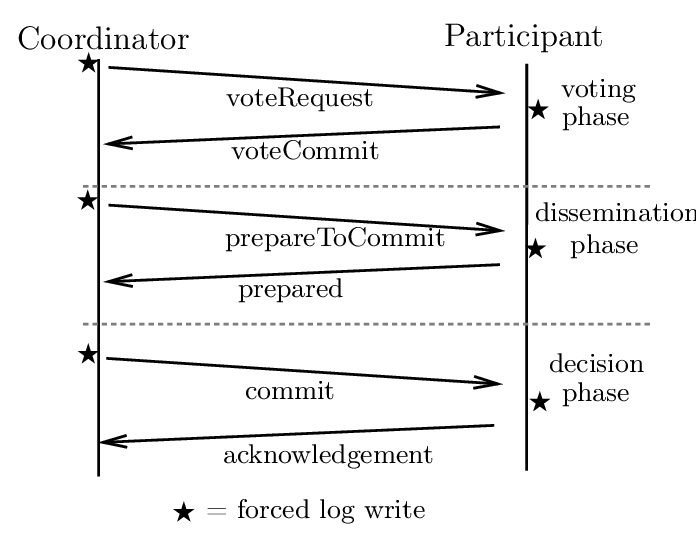
\includegraphics[scale=0.14]{figures/3PC.png}
    \caption{Three-Phase Commit Protocol (3PC)}
    \label{fig:3pc}
\end{figure}
\begin{itemize}
\item Introduces an additional phase for enhanced fault tolerance.
\item Facilitates progressive commit decisions to mitigate risks.
\item Coordinator solicits participant readiness to commit.
\item Confirms commit readiness before final decision.
\item Coordinator makes a definitive commit or abort decision.
\end{itemize}

\end{frame}


\section{Motivation/Importance}
\begin{frame}
\frametitle{Motivation/Importance}
\framesubtitle{Navigating Consensus: The Distributed Commit Challenge}
The distributed commit problem is pivotal in ensuring agreement among system nodes on transaction outcomes in distributed systems. It poses philosophical questions about autonomy versus consensus and is addressed by models like the commit protocols, despite limitations. Its applications are widespread, but its complexity stems from reconciling consensus in fault-prone distributed environments, emphasizing the need for nuanced solutions.
\end{frame}

\section{Background/Model/Definitions/Previous Works}


\subsection{Model, Definitions}

\frame{
\frametitle{Model, Definitions}
\framesubtitle{Formal definition of Commit Protocol}

\textbf{Coordinator:} Initiates and coordinates the distributed transaction by communicating with participating nodes to ensure consistency.

\textbf{Nodes:}  Participate in the distributed transaction by responding to the coordinator's messages, executing transactional operations, and maintaining transactional integrity.

\textbf{Prepare Phase:} The coordinator sends a "prepare" message to all participants, asking if they are ready to commit the transaction. Each participant replies with either a "yes" or "no" message.

\textbf{Can Commit Phase:}  The coordinator asks participants if they can commit the transaction without actually committing it. Participants reply with "yes" or "no".

\textbf{Commit Phase:} If all participants reply "yes" during the "can commit" phase, the coordinator proceeds with the commit phase; otherwise, it aborts the transaction.
}

\subsection{Background, Previous Works}
\begin{frame}{Background}

\begin{itemize}
    \item The Two-Phase Commit protocol ensures atomicity in distributed systems by employing two phases: prepare and commit, as introduced by Gray 1978 \cite{gray_1978}.

    \item The Three-Phase Commit protocol enhances the Two-Phase Commit by introducing a pre-commit phase, reducing the likelihood of blocking in case of coordinator failure, as proposed by Skeen 1981\cite{skeen_1981}
\end{itemize}

\end{frame}




\section{Contribution}
\subsection{Main Point 1}
\begin{frame}{Main Point 1: A Figure}
\framesubtitle{Abstract the Major Results}
Describe the key results of the paper. You may present the statements of the major theorems, but not their proofs. You will probably have to get a little technical here, but do so gradually and carefully.

\begin{figure}
    \centering
    \includegraphics[scale=0.5]{figures/Chick1.png}
    \caption{Awesome Image}
    \label{fig:awesome_image}
\end{figure}
\note{
}
\end{frame}


\subsection{Main Point 2}

\begin{frame}
\frametitle{An Example Distributed Algorithm}
\framesubtitle{Blind Flooding}


Blind flooding on an undirected graph is presented in Algorithm~\ref{alg:blindflooding}.

\begin{center}
\begin{algorithm}[H]
	\scriptsize
	\def\algorithmlabel{BlindFlooding}
    \caption{\algorithmlabel\ algorithm}
    \label{alg:blindflooding}
    \begin{algorithmic}[1]
    	\Implement {\algorithmlabel}{cf} 
    	\Use {LinkLayerBroadcast} {lbc} 
    	\Events{Init, MessageFromTop, MessageFromBottom}
	\Need {}

        \Event {Init}{}
        		
        \Event{MessageFromBottom} { $m$ }
        		\Trig{lbc}{Broadcast} { $m$  }
        		
        \Event{MessageFromTop} { $m$ }	
        		\Trig{lbc}{Broadcast} { $m$  }
    \end{algorithmic}
\end{algorithm}
\end{center}


\end{frame}

\begin{frame}
\frametitle{Main Point 2}
\framesubtitle{Explain the Significance of the Results}
Pause, and explain the relationships between the formal theorems that you have just presented and the informal description that you gave in the Introduction. Make it clear to the audience that the results do live up to the advance publicity. If the statements of the theorems are very technical then this may take some time. It is time well-spent.

\end{frame}

\subsection{Main Point 3}
\begin{frame}
\frametitle{Main Point 3}
\framesubtitle{Sketch a Proof of the Crucial Results}
The emphasis is on the word ``sketch''. Give a very high-level description of the proofs, emphasizing the proof structure and the proof techniques used. If the proofs have no structure (in which case it may be assumed that you are not the author of the paper), then you must impose one on them. Gloss over the technical details. It is a good idea to point them out but not to explore them.
\end{frame}


\section{Experimental results/Proofs}

\subsection{Main Result 1}
\begin{frame}
\frametitle{Main Result 1}
\framesubtitle{}
Choose \textbf{just the key results}. They should be important, non-trivial, should give the flavour of the rest of the technical details and should be presentable in a relatively short period of time. Use figures instead of tables instead of text.

Better to present 10\% the entire audience gets than 90\% nobody gets
\end{frame}


\subsection{Main Result 2}
\begin{frame}
\frametitle{Main Result 2}
\framesubtitle{Try a subtitle}
\begin{itemize}
\item Make sure your notation is clear and consistent throughout the talk. Prepare a slide that explains the notation in detail, in case that is needed or if somebody asks.
\item Always label all of your axes on graphs; use short but helpful captions on figures and tables. It is also very useful to have an arrow on the side which clearly shows which direction is considered better (e.g., "up is better").
\item If you have experimental results, make sure you clearly present the experimental paradigm you used, and the details of your methods, including the number of trials, the specific analysis tools you applied, significance testing, etc.
\item The talk should contain at least a brief discussion of the limitations and weaknesses of the presented approach or results, in addition to their strengths. This, however, should be done in an objective manner -- don't enthusiastically put down your own work.
\end{itemize}
\end{frame}


\subsection{Main Result 3}
\begin{frame}
\frametitle{Main Result 3}
\framesubtitle{}
\begin{itemize}
\item If time allows, the results should be compared to the most related work in the field. You should at least prepare one slide with a summary of the related work, even if you do not get a chance to discuss it. This will be helpful if someone asks about it, and will demonstrate your mastery of the material.
\item Spell check again.
\item Give for each of the x-axis, y-axis, and z-axis
\item Label, unit, scale (if log scale)
\item Give the legend
\item Explain all symbols
\item Take an example to illustrate a specific point in the figure
\end{itemize}
\end{frame}



\section{Conclusions}
\begin{frame}
\frametitle{Conclusions}
\framesubtitle{Hindsight is Clearer than Foresight}
Advices come from \cite{spillman2000present}.
\begin{itemize}
\item You can now make observations that would have been confusing if they were introduced earlier. Use this opportunity to refer to statements that you have made in the previous three sections and weave them into a coherent synopsis. You will regain the attention of the non- experts, who probably didn’t follow all of the Technicalities section. Leave them feeling that they have learned something nonetheless.
\item Give Open Problems It is traditional to end with a list of open problems that arise from your paper. Mention weaknesses of your paper, possible generalizations, and indications of whether they will be fruitful or not. This way you may defuse antagonistic questions during question time.
\item Indicate that your Talk is Over
An acceptable way to do this is to say “Thank-you. Are there any questions?”\cite{einstein}
\end{itemize}

\end{frame}

\section*{References}
\begin{frame}{References}
\tiny
\bibliographystyle{IEEEtran}
\bibliography{refs}
\end{frame}

\begin{frame}{How to prepare the talk?}
Please read \url{http://larc.unt.edu/ian/pubs/speaker.pdf}
\begin{itemize}
\item The Introduction:  Define the Problem,    Motivate the Audience,    Introduce Terminology,    Discuss Earlier Work,    Emphasize the Contributions of your Paper,    Provide a Road-map.
\item The Body:    Abstract the Major Results, Explain the Significance of the Results, Sketch a Proof of the Crucial Results
\item Technicalities: Present a Key Lemma, Present it Carefully
\item The Conclusion: Hindsight is Clearer than Foresight, Give Open Problems, Indicate that your Talk is Over
\end{itemize}

\note{
\begin{itemize}
\item The Introduction:  Define the Problem,    Motivate the Audience,    Introduce Terminology,    Discuss Earlier Work,    Emphasize the Contributions of your Paper,    Provide a Road-map.
\item The Body:    Abstract the Major Results, Explain the Significance of the Results, Sketch a Proof of the Crucial Results
\item Technicalities: Present a Key Lemma, Present it Carefully
\item The Conclusion: Hindsight is Clearer than Foresight, Give Open Problems, Indicate that your Talk is Over 
\end{itemize}
}
\end{frame}



\thankslide




\end{document}